\chapter{Introduction}\label{intro}

From a genetics point of view, the process of \gls{carcinogenesis} is operated and characterised by mutations \citep{Stratton2009}. While every cancer has a different set of mutations, certain mutation patterns have been found exclusive to several cancer types \citep{Alexandrov2013,Polak2015,Campbell2020}. Since all cancers originate from a normal cell \citep{Hanahan2011HallmarksGeneration}, it is likely that the patterns of cancer \gls{mutagenesis}, to some extent, reflect the mutation tendency in the original cell type. During its development, the phenotype of a cancer sample could diverge from that of the original cell, but virtually all mutations prior to the divergence remain in the cancer genome. These divergence events can be caused by driver mutations, which promote cancer cell proliferation \citep{Pon2015}. An average cancer sample consists of only about 4-5 drivers, the rest are passenger mutations, which have neutral effects on the cancer progress \citep{Campbell2020}. Together, the whole history of mutations in a cancer sample helps characterise its mutation profile (Figure \ref{fig:drivers_demo}). The mutation profile more or less reflects the mechanism of mutagenesis, which offers a great opportunity to study cancer. Accordingly, this project seeks to analyse the invaluable information extracted from the cancer mutation profiles, which could potentially help guiding cancer treatment. Furthermore, the project seeks to exploit this information to predict cancer types by training a \gls{classifier} that only relies on genomic sequencing data. In the long term, such a classifier could be an additional diagnostic tool to existing clinical approaches such as cytology or biopsy \citep{Stone1995Biopsy:Pitfalls}. In this era of next generation sequencing, liquid biopsies are gaining interest as a powerful non-invasive method for early cancer diagnosis because they involve screening for circulating tumour DNA in the blood rather than obtaining samples from a suspected local tissue \citep{Chen2019Next-generationDetection}. Developing a genome-based classifier model means that liquid biopsies could inform not only whether a cancer is present, but also where and what cancer is occurring at an early stage.  

Regarding the scope of the project, two aspects of of a cancer mutation profile were studied: where mutations tend to be found in the genome (hereafter the Genomic Location Effect, GLE) and what \gls{base} changes tend to be found in which genomic sequence context (hereafter the Sequence Context Effect, SCE). Secondly, the project is limited to point mutations, which are the most abundant type of mutations in cancer \citep{Alexandrov2020}. Thirdly, due to the different mutation rates between drivers and passengers, they should be considered separately - this project focuses on passenger mutations \citep{McFarland2014Tug-of-warProcesses}. Finally, this project only investigates \glspl{sommut} as opposed to \glspl{germline_mut}, acknowledging that germline mutations could themselves be a risk factor of cancer. The reason for this is that germline mutations reflect a process that definitely occurs prior to carcinogenesis. Strictly speaking, somatic mutations can also occur before carcinogenesis, but they are still arguably the consequence of the environment in which cancer develops (Figure \ref{fig:drivers_demo}). 

\begin{figure}[h!]
    \centering
    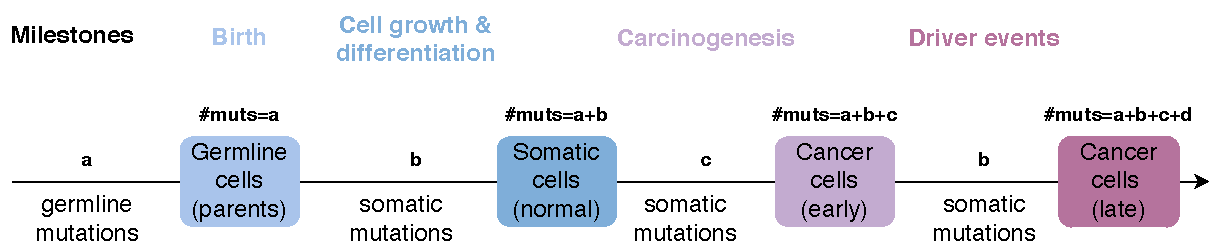
\includegraphics[scale=0.78]{graphics/drivers_demo.pdf}
    \caption{\textbf{Timeline of a carcinogenesis process.} Mutations are generally retained in the genome after each stage of carcinogenesis, even though carcinogenesis and driver events could change the phenotype of the cells. Together, all mutations available in a cancer cell make up it mutation profile. For the purpose of this project, only somatic mutations are considered because germline mutations occur prior to birth and are not the product of the environment of the differentiated cells in which cancer develop.}
    \label{fig:drivers_demo}
\end{figure}


To outline this chapter, section \ref{intro:gle} and \ref{intro:sce} review what is known about GLE and SCE, respectively. Section \ref{intro:ml} then briefly introduces the statistical approaches used to study GLE and SCE, as well as how they can be used to train a machine learning classifier.

\section{Genomic location effect (GLE)}
\label{intro:gle}
Certain regions of the genome are more prone to mutations than others. These regions are distributed at different locations of the genome in different cell-types \citep{Polak2015}. This is because different cells have different chromatin structures \citep{Abascal2020ExpandedGenomes}, which are determined by how hidden DNA is in the chromatin complex across the genome. The accessibility of DNA to factors such as transcription, mutagens and repair systems can be measured by Dnase I hypersensitivity \citep[DHS;][]{Liu2019AApplications}. Highly accessible DNA means open chromatin status, and vice versa. Because mutation is the product of both \glspl{mutagen} and repairs \citep{Ripley2001Mutation}, it is reasonable to expect that the most vulnerable regions are those with strong mutagens and weak repairs. In reality, DNA in the closed chromatin region is less exposed to both mutagens and repairs \citep[Figure \ref{fig:chromatin_demo};][]{Teng1997ExcisionSequences, Morse2002PhotoreactivationCerevisiae}. However, it has been reported that closed chromatin regions are more likely to harbour mutations than open regions \citep{Polak2015,Prendergast2007ChromatinGenome}, suggesting that the repair effect is generally stronger. The diversity of chromatin structures and of how mutagen/repair system works in different cells makes genomic location of mutations (GLE) an important characteristic of the cancer mutation profile. Chapter \ref{gle} of this project seeks to formally test to which degree GLE differs in closed \textit{v.s.} open chromatin regions for each cancer. Chapter \ref{gle} also evaluates the difference in GLE between cancers, without prior knowledge of chromatin status. This serves to assess the information content available in GLE so it can be exploited to predict cancer types in Chapter \ref{ml}.

\begin{figure}[h!]
    \centering
    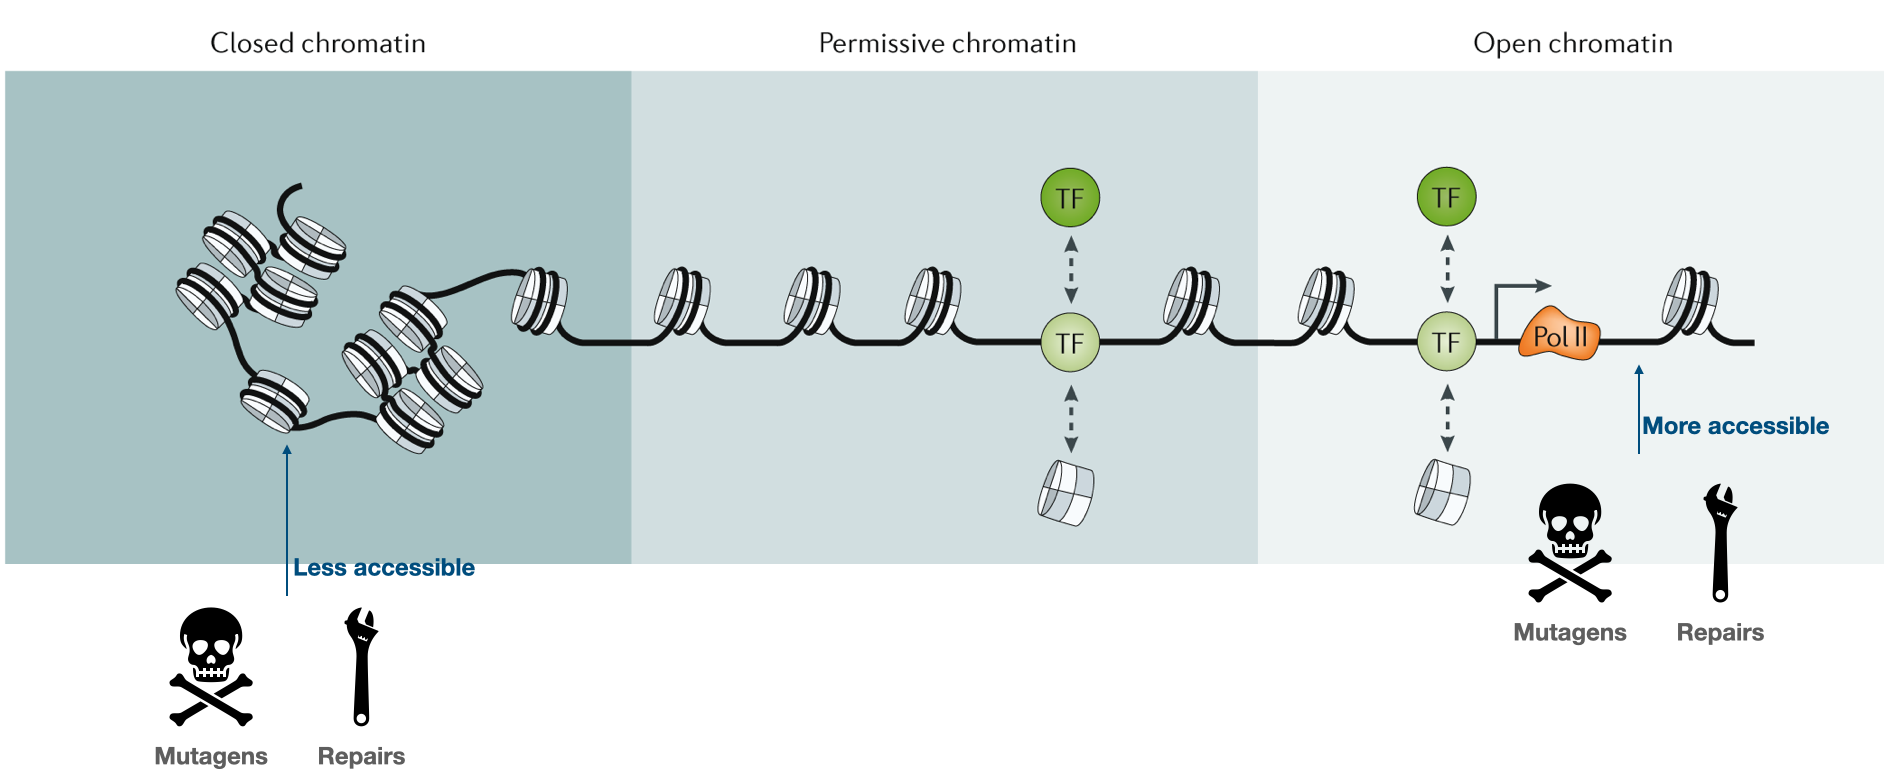
\includegraphics[scale=0.24]{graphics/chromatin_demo.png}
    \caption{\textbf{The distribution of mutations across the genome is hypothetically influenced by cell chromatin structure.} DNA in closed chromatin regions is not accessible to both mutagens and repairs, and is more prone to mutations. Different cell types have different chromatin structures as well as different repair systems, making genomic location effect (GLE) a potential factor that makes a cancer distinct from another. Figure modified from \citet{Klemm2019ChromatinEpigenome}. TF means transcription factor, Pol II means polymerase II}.
    \label{fig:chromatin_demo}
\end{figure}


\section{Sequence context effect (SCE)}
\label{intro:sce}

Each cancer develops under the influence of different mutagenic processes, giving rise to diverse mutation compositions. These processes include, but are not limited to UV light \citep[known in skin melanoma;][]{Mohania2017}, the intrinsic cellular APOBEC deaminase activity \citep[\textit{e.g.} in B cells;][]{Kuppers2005MechanismsPathogenesis} and defective repairs \citep[\textit{e.g.} mutated \textit{BRCA} genes in breast cancer;][]{Navasardyan2021YY1TNBC}. \citet{Alexandrov2013, Alexandrov2020} showed that some processes were associated with certain mutation signatures. For instance, the signature SBS4, where there is an excess of C$\rightarrow$A mutations in the context of C[C$\rightarrow$A]A and C[C$\rightarrow$A]C over any other mutations, were only detected in tobacco smoke linked cancers such as liver hepatocellular carcinoma, lung adenocarcinoma and lung squamous cell carcinoma. As such, similar to \gls{gle}, mutation composition is also an important characteristic of the cancer mutation profile. In inspecting mutation composition, one should stay aware that mutations are usually closely linked with the \glspl{base} next to them \citep{Zhu2017}. A well known example is that the C$\rightarrow$T mutations tend to occur in the [C$\rightarrow$T]G context. One possible explanation is that proteins, be they repairs or mutagens, interact with DNA with high specificity (Figure \ref{fig:motif_demo}). While it is a common practice to analyse mutation compositions in the 3-mer (3 base) context, evidence showed that bases beyond 3-mer can also influence whether mutations occur or not \citep{Zhu2017,Zhu2020}. This project seeks to explore the information content available in different sequence context sizes (SCE). Chapter \ref{sce} breaks SCE into two separate analyses: the base change and the flanking bases. Chapter \ref{ml} then uses both sources of information to train a cancer classification model.  

\begin{figure}[h!]
    \centering
    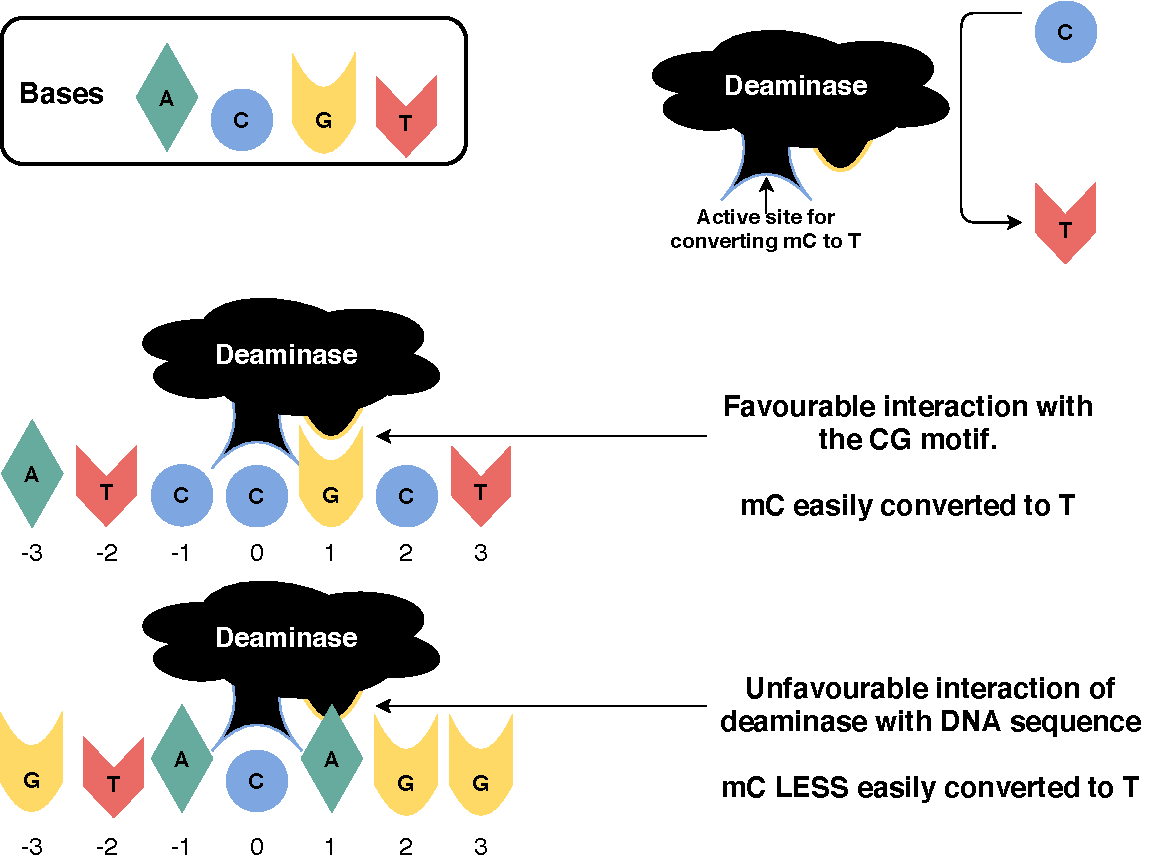
\includegraphics[scale=0.78]{graphics/motif_demo.pdf}
    \caption{\textbf{Mutations are closely linked with the bases next to them}. The schematic diagram depicts an example of hypothetical scenarios that could explain why this is the case. Here, a deaminase protein, which converts methylated C into T, interacts with DNA such that certain sequence contexts make the conversion more feasible than others. While many publications focus on the 3-mer context of mutations (pos -1, 0 and 1), which includes the base change and two bases immediately next to it, evidence shows that bases outside the 3-mer could still be influential. Part of this project seeks to explore the information content available in larger sequence contexts than 3-mers.}
    \label{fig:motif_demo}
\end{figure}


\section{Computational approaches for exploiting GLE and SCE to predict cancers}
\label{intro:ml}

The release of the \gls{pcawg} project \citep{Campbell2020} has made studying cancer genomics and developing cancer classification models on a large scale feasible. PCAWG is an international collaboration that produced whole genomic sequencing data for 2605 primary tumours of 38 cancer types. Nevertheless, besides data availability, it is equally important to have satisfactory computational tools for data analysis. Developing such tools requires understanding the nature of the data, which this project approaches from two ends (see project outline in Figure \ref{}). First, conventional statistical tools are recruited to detect signals in mutation data (\gls{gle} in Chapter \ref{gle}; \gls{sce} in Chapter \ref{sce}). Second, Chapter \ref{ml} trials different measures and data representations to train the classifiers. The idea is that the more accurate the classifier, the better the assumptions imposed by its data representations could capture the nature of the data. Moreover, the long term goal is to be able to apply the model to unseen data, such as the tumour genome of a new cancer patient. Therefore, Chapter \ref{ml} adopts a standard \gls{ml} cross-validation procedure \citep{Zengyou2015DataApplications}, meaning part of the data is used to train the model, the rest is held out to validate model performance\footnote{Details in }. Overall, the project shows that both GLE and SCE are informative factors that could be used to identify cancer from a \gls{mut_profile}. Each factor alone provides reasonably high predictive power, but the performance is even greater when combining them in a joint model.

\section{Aims}

\begin{itemize}
    \item 
\end{itemize}